
\begin{frame}{What is Document-level Machine Translation}
	\begin{figure}
	\centering
	\begin{minipage}{.4\textwidth}
		\centering
		\textbf{Sentence-level MT}\par\medskip
		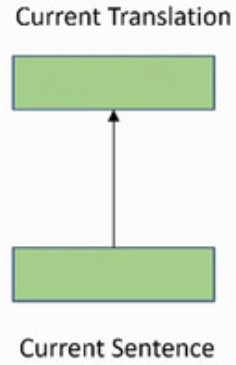
\includegraphics[width=.4\linewidth]{Images/dlmt}
	\end{minipage}%
	\begin{minipage}{.6\textwidth}
		\centering
		\textbf{Document-level MT}\par\medskip
		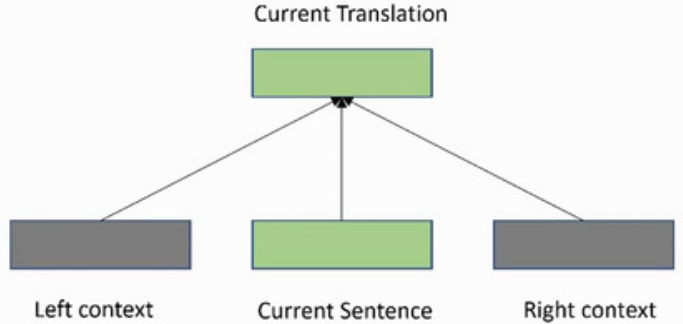
\includegraphics[width=.85\linewidth]{Images/slmt}
	\end{minipage}
	\end{figure}	
\end{frame}

\begin{frame}{Document-level MT $\leftrightarrow$ Context-aware MT}
	\begin{figure}
	\centering
	\begin{minipage}{.4\textwidth}
		\centering
		\textbf{Context-agnostic MT}\par\medskip
		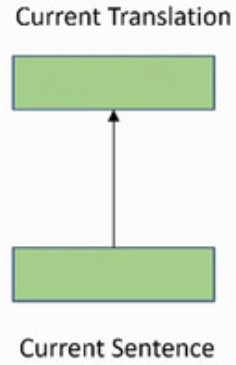
\includegraphics[width=.4\linewidth]{Images/dlmt}
	\end{minipage}%
	\begin{minipage}{.6\textwidth}
		\centering
		\textbf{Context-aware MT}\par\medskip
		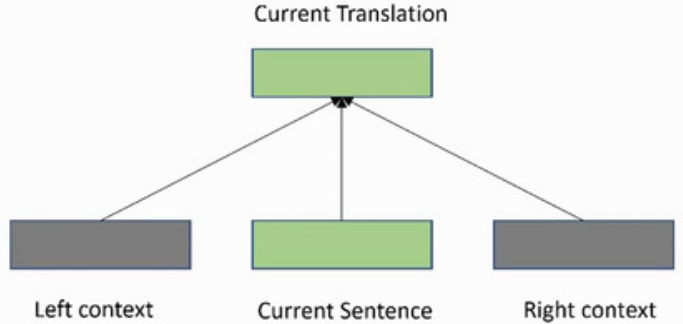
\includegraphics[width=.85\linewidth]{Images/slmt}
	\end{minipage}
	\end{figure}	
\end{frame}

\begin{frame}{Sentence-level MT is inconsistent}
	\begin{center}
		\onslide<3->{%
			\begin{minipage}{0.75\textwidth}
				\RaggedRight
				\textbf{A}: Nous avons refait l'exercice avec les m\^emes etudiants. \\
				\ \ \ \ Que  pensez-vous qu'il est \textcolor{blue}{alors} arriv\'e ?
			\end{minipage}
			\bigskip
		}
		\onslide<1->{%
			\begin{minipage}{0.75\textwidth}
				\RaggedRight
				\textbf{B}: \textcolor{blue}{L\`a},  ils  comprenaient  l'importance de la coh\'esion lexicale.
			\end{minipage}
			\bigskip
		}
		\onslide<2->{%
			\textbf{SENTENCE-LEVEL TRANSLATION}
			\medskip
			
			\begin{minipage}{0.75\textwidth}
				\RaggedRight
				\textbf{B}: \textcolor{red}{There} they understood the importance of lexical cohesion.
	
			\end{minipage}
			\bigskip
		}
		\onslide<4->{%
			\textbf{CONTEXT-AWARE TRANSLATION}
			\medskip
			
			\begin{minipage}{0.75\textwidth}
				\RaggedRight
				\textbf{B}: \textcolor{green}{Now}, they understood the importance of lexical cohesion.
			\end{minipage}
		}
	\end{center}
\end{frame}

\begin{frame}{How bad is it?}
	\onslide<1->{%
		\cite{voita_when_2019} undertake a  human  study  on context agnostic translation :
			\begin{itemize}
				\item 2000 pairs of consecutive English sentences (S1 + S2) from OpenSubtitles2018
				\item translate to Russian with Transformer model \cite{vaswani_attention_2017}
			\end{itemize} 
	} 
	\onslide<2->{
	\begin{figure}
		\centering
		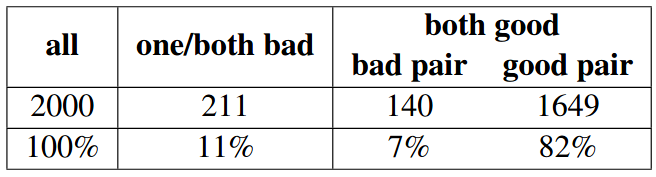
\includegraphics[width=0.7\linewidth]{Images/inconsistent_sentences}
		\label{fig:inconsistentsentences}
	\end{figure}
	}
	
\end{frame}

\begin{frame}{Which kind of inconsistencies?}
	\begin{figure}
		\centering
		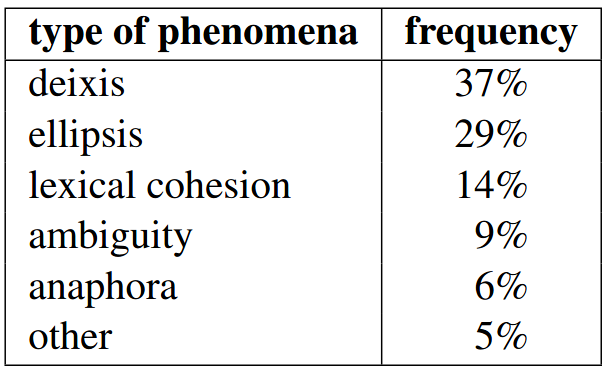
\includegraphics[width=0.7\linewidth]{Images/phenomena}
		\caption{Types of phenomena causing discrepancies in context-agnostic  translation  of  consecutive  sentences when placed in the context of each other.}
		\label{fig:phenomena}
	\end{figure}	
\end{frame}

\begin{frame}{Objectives}
	\begin{itemize}
		\item<+(1)-|alert@+(1)> \textbf{Design translation models} that solve discrepancies by taking context into account;
		\item<+(1)-|alert@+(1)> \textbf{Evaluate such models} in a proper way;
	\end{itemize}
	
\end{frame}
